We now impose integrality. In this section, $\Gamma=\operatorname{SL}_2(\mathbb Z)$ and its effective image is $\overline\Gamma=\operatorname{PSL}_2(\mathbb Z)$. We will construct a fundamental domain: a region whose translates cover $\mathbb H$ and whose interior translates do not overlap. The effective group indexes these translates, since $\gamma$ and $-\gamma$ act identically.

\begin{proposition}[Discreteness and properness]\label{modular.properness}
The subgroup $\Gamma$ is discrete in $G$. For compact subsets $B_1,B_2\subset\mathbb H$, there are only finitely many $\gamma\in\Gamma$ for which $\gamma B_1\cap B_2\ne\varnothing$. In particular, point stabilizers are finite, and the effective action is properly discontinuous in this compact-set sense.
\end{proposition}

\begin{proof}
An integer matrix is isolated in the space of real matrices, and a bounded set contains only finitely many integer matrices. If $\gamma\cdot z=w$ with $z\in B_1,w\in B_2$, the Iwasawa section $s(z)=n(\operatorname{Re}z)a(\operatorname{Im}z)$ gives
\[
 \gamma=s(w)k\,s(z)^{-1}\quad\text{for some }k\in K.
\]
All such products lie in the compact image of $B_2\times K\times B_1$ under this continuous map. That compact set contains finitely many integer matrices. Apply the result to singleton sets to obtain the assertion about stabilizers.
\end{proof}

\begin{proposition}[Generators]\label{modular.generators}
The matrices
\[
 S=\begin{pmatrix}0&-1\\1&0\end{pmatrix},\qquad
 T=\begin{pmatrix}1&1\\0&1\end{pmatrix}
\]
generate $\Gamma$.
\end{proposition}

\begin{proof}
First see what left multiplication does to the rows of an arbitrary matrix $\gamma=\begin{smallpmatrix}a&b\\c&d\end{smallpmatrix}$. Direct multiplication gives
\begin{equation}\label{eq:modular-row-operations}
 S\gamma=\begin{pmatrix}-c&-d\\a&b\end{pmatrix},\qquad
 T^q\gamma=\begin{pmatrix}a+qc&b+qd\\c&d\end{pmatrix}
 \quad(q\in\mathbb Z).
\end{equation}
Thus $S$ exchanges the two rows and negates the new first row, while $T^q$ adds $q$ times the second row to the first. These operations preserve integrality and determinant one.

We now use these row operations to reduce the first column. Suppose $c\ne0$. Choose an integer $q$ nearest to $-a/c$, so
\[
 |a+qc|\leq\frac{|c|}{2}<|c|.
\]
Apply $T^q$ and then $S$. The row-operation formulas \eqref{eq:modular-row-operations} give
\[
 ST^q\gamma=\begin{pmatrix}-c&-d\\a+qc&b+qd\end{pmatrix}.
\]
In particular, the first column changes by
\[
 \begin{pmatrix}a\\c\end{pmatrix}
 \longmapsto
 \begin{pmatrix}a+qc\\c\end{pmatrix}
 \longmapsto
 \begin{pmatrix}-c\\a+qc\end{pmatrix}.
\]
This is the Euclidean algorithm: subtract an integer multiple and exchange the entries. The absolute value of the bottom entry strictly decreases whenever it is nonzero. Since it is a nonnegative integer, after finitely many steps it is zero.

Finally, a determinant-one integer matrix with bottom-left entry zero has the form
\[
 \begin{pmatrix}\varepsilon&b\\0&\varepsilon\end{pmatrix}
 =\varepsilon T^{\varepsilon b},\qquad \varepsilon\in\{1,-1\}.
\]
Both possibilities belong to the subgroup generated by $S,T$, because $S^2=-I$. All reduction steps were products of $S$ and powers of $T$, so reversing them expresses the original $\gamma$ in these generators.
\end{proof}

\begin{proposition}[Generator actions and relations]\label{modular.generator-relations}
The generators act by $S\cdot z=-1/z$ and $T\cdot z=z+1$. They satisfy $S^2=(ST)^3=-I$. Consequently $\overline S$ has order $2$ and $\overline{ST}$ has order $3$ in $\overline\Gamma$.
\end{proposition}

\begin{proof}
The actions follow by substituting the matrix entries into the fractional formula. For the relations, multiply:
\[
 S^2=-I,\qquad
 ST=\begin{pmatrix}0&-1\\1&1\end{pmatrix},\qquad
 (ST)^2=\begin{pmatrix}-1&-1\\1&0\end{pmatrix},\qquad
 (ST)^3=-I.
\]
Neither $S$ nor $ST$ is central. Their effective orders therefore divide $2$ and $3$, respectively, and are not $1$, proving the claim. These relations are sufficient for our purposes; a complete group presentation is not asserted here.
\end{proof}

\begin{definition}[A closed fundamental domain]\label{modular.fundamental-domain-definition}
In this definition, let $\Gamma$ be an arbitrary discrete subgroup of $\operatorname{PSL}_2(\mathbb R)$ acting on $\mathbb H$. For a set $E\subset\mathbb H$, write $\gamma\cdot E=\{\gamma\cdot z:z\in E\}$. A closed fundamental domain for this action is a closed set $F\subset\mathbb H$ such that:
\begin{itemize}
\item its interior $F^\circ$ is nonempty and connected, and $F=\overline{F^\circ}$, with closure taken in $\mathbb H$;
\item the translates cover: $\mathbb H=\bigcup_{\gamma\in\Gamma}\gamma\cdot F$;
\item distinct translates have disjoint interiors: $(\gamma\cdot F^\circ)\cap F^\circ=\varnothing$ for every $\gamma\in\Gamma\setminus\{1\}$.
\end{itemize}
Boundary points may have several representatives in $F$. One obtains the quotient by identifying boundary points in the same orbit. We use the closed-domain convention here; authors who call $F^\circ$ the fundamental domain express the covering condition using its closure. A set containing exactly one point of every orbit is a separate choice of representatives.
\end{definition}

\begin{definition}[The standard modular domain]\label{modular.fundamental-region}
Set
\[
 \mathcal F=\{x+iy\in\mathbb H: |x|\leq\tfrac12,\ |x+iy|\geq1\},
 \qquad
 \rho=-\tfrac12+\tfrac{\sqrt3}{2}i.
\]
Its lower boundary is the unit-circle arc from $\rho$ to $\rho+1$, and its two vertical sides extend upward from these endpoints. Its interior $\mathcal F^\circ$ is given by both inequalities strict. We will prove that $\mathcal F$ is a closed fundamental domain for $\overline\Gamma$.
\end{definition}

The \hyperref[modular.domain-diagram]{fundamental-domain diagram} labels the sides that will be identified. The translation $T$ pairs the left vertical side with the right, and $S$ pairs the left half of the circular arc with the right. The dashed segment from $i$ upward divides the domain into two halves; it is not a boundary of $\mathcal F$. It will help us describe the topology of the quotient in \hyperref[modular.quotient-topology]{Section 1.7}.

\begin{figure}[!htb]
\begin{center}
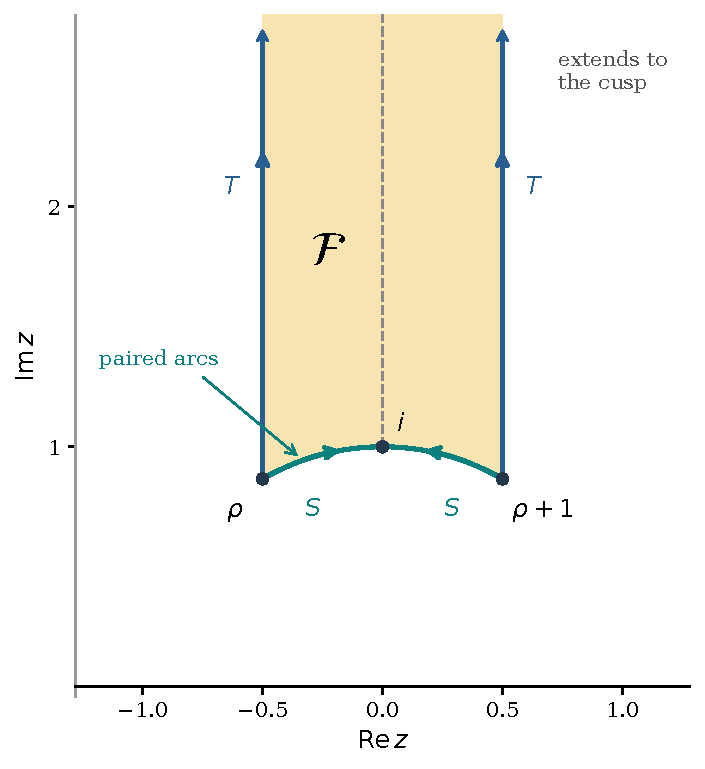
\includegraphics[width=0.55\linewidth]{volumes/Volume01/A/chapters/Chapter01/sections/Section06/figures/fundamental-domain.pdf}
\end{center}
\caption{The closed modular fundamental domain $\mathcal F$. Arrows with the same label indicate paired sides: $T$ sends the left vertical side to the right, and $S$ sends the arc from $\rho$ to $i$ to the arc from $\rho+1$ to $i$. The points $\rho$ and $\rho+1$ are identified; $i$ is fixed by $S$. The domain extends upward without a top edge. The dashed internal segment will divide its compactification into two disks.}
\label{modular.domain-diagram}
\end{figure}

\begin{lemma}[The denominator bound]\label{modular.denominator-bound}
For $z\in\mathcal F$ and $(c,d)\in\mathbb Z^2\setminus\{(0,0)\}$,
\begin{equation}\label{eq:modular-denominator-bound}
 |cz+d|\geq1.
\end{equation}
If $z\in\mathcal F^\circ$ and $c\ne0$, then $|cz+d|>1$.
\end{lemma}

\begin{proof}
Write $z=x+iy$. The defining inequalities for $\mathcal F$ give
\begin{equation}\label{eq:modular-height-lower-bound}
 y^2\geq1-x^2\geq\frac34.
\end{equation}
If $c=0$, then $d$ is a nonzero integer, so $|cz+d|=|d|\geq1$.

If $|c|\geq2$, use the height lower bound \eqref{eq:modular-height-lower-bound}:
\[
 |cz+d|^2=(cx+d)^2+c^2y^2\geq c^2y^2\geq3>1.
\]
If $|c|=1$, changing both signs reduces to $c=1$. Since $|x|\leq1/2$ and $d\in\mathbb Z$,
\begin{equation}\label{eq:modular-unit-row-bound}
 |z+d|^2=|z|^2+2dx+d^2\geq1-|d|+d^2\geq1.
\end{equation}
For the last inequality, $d^2-|d|=|d|(|d|-1)\geq0$ because $|d|$ is a nonnegative integer. These cases prove the bound. If $z\in\mathcal F^\circ$, then $|z|^2>1$, making the first inequality in the unit-row estimate \eqref{eq:modular-unit-row-bound} strict as well.
\end{proof}

\begin{theorem}[The modular fundamental domain]\label{modular.fundamental-domain}
The set $\mathcal F$ is a closed fundamental domain for $\overline\Gamma$. More precisely, every $\Gamma$-orbit meets $\mathcal F$, and if $z\in\mathcal F^\circ$ and $\gamma\cdot z\in\mathcal F$, then $\gamma\in Z$.
\end{theorem}

\begin{proof}
First we move an arbitrary point $z=x+iy$ into $\mathcal F$. Among primitive integer pairs $(c,d)$, choose one minimizing $|cz+d|$. Such a minimum exists: $(0,1)$ gives value $1$, while $|cz+d|\leq1$ implies
\[
 |c|y\leq1,\qquad |cx+d|\leq1.
\]
The first inequality bounds the integer $c$, and for each such $c$ the second bounds the integer $d$. Thus only finitely many pairs need to be considered. The minimum is positive because $z\in\mathbb H$.

By B\'ezout, complete the minimizing pair to the bottom row of a matrix $\gamma\in\Gamma$. The imaginary-part identity \eqref{eq:mobius-imaginary-part} gives
\begin{equation}\label{eq:modular-orbit-height}
 \operatorname{Im}(\gamma\cdot z)=\frac{\operatorname{Im}z}{|cz+d|^2}.
\end{equation}
Every bottom row of a determinant-one integer matrix is primitive, so $w=\gamma\cdot z$ has maximal height in its orbit. Translate $w$ by a power of $T$ to obtain $|\operatorname{Re}w|\leq1/2$ without changing its height. If $|w|<1$, then
\[
 \operatorname{Im}(S\cdot w)=\frac{\operatorname{Im}w}{|w|^2}>\operatorname{Im}w,
\]
contradicting maximality. Thus $w\in\mathcal F$, proving that the translates cover $\mathbb H$.

Next we prove uniqueness when one representative is interior. Suppose $z,w=\gamma\cdot z$ both lie in $\mathcal F$. The denominator bound \eqref{eq:modular-denominator-bound} and the orbit-height formula \eqref{eq:modular-orbit-height} give $\operatorname{Im}w\leq\operatorname{Im}z$. Apply the same argument to $\gamma^{-1}$ at $w$ to get the reverse inequality. Therefore
\begin{equation}\label{eq:modular-domain-height-equality}
 \operatorname{Im}w=\operatorname{Im}z,\qquad |cz+d|=1.
\end{equation}
If $z$ is interior, the strict denominator bound forces $c=0$. The determinant then gives $\gamma=\pm T^m$ for some integer $m$. Its action is $w=z+m$. Since $\operatorname{Re}z\in(-1/2,1/2)$ and $\operatorname{Re}w\in[-1/2,1/2]$, necessarily $m=0$. Thus $\gamma\in Z$. In the effective group, this says that a nonidentity element cannot carry an interior point into $\mathcal F$, so distinct interior translates are disjoint.

Finally, $\mathcal F$ is closed in $\mathbb H$ by its weak inequalities. Its interior is the nonempty region described by strict inequalities, and every boundary point is a limit of interior points, by moving slightly inward from a vertical side and upward from the circular arc. Its interior is connected: two interior points can each be moved vertically to a common height greater than $1$, joined horizontally within the strip, and then joined back to the original heights. These properties verify the remaining conditions in the \hyperref[modular.fundamental-domain-definition]{definition of a closed fundamental domain}.
\end{proof}

\begin{proposition}[Boundary identifications]\label{modular.boundary-identifications}
Distinct boundary points of $\mathcal F$ are identified only by the following side pairings and their consequences at the endpoints: $T$ pairs the vertical sides, and $S$ pairs the two halves of the circular arc.
\end{proposition}

\begin{proof}
Let $z,w=\gamma\cdot z$ lie in $\mathcal F$. The height and denominator equalities \eqref{eq:modular-domain-height-equality} give $|cz+d|=1$ and equal imaginary parts.

If $c=0$, the transformation is translation by an integer. The only distinct points in the closed strip related by such a translation lie on opposite vertical sides and differ by $1$. They are paired by $T$ or $T^{-1}$.

If $c\ne0$, the proof of the denominator bound forces $|c|=1$. Up to a central sign take $c=1$. If $d=0$, equality requires $|z|=1$. The determinant gives $b=-1$, so $\gamma=T^aS$. On the unit-circle arc, $S\cdot z=-\overline z$. Both $S\cdot z$ and $w=S\cdot z+a$ lie in the closed strip, so $a=0$ except possibly at its endpoints. Thus $S$ pairs the two halves of the arc and fixes their meeting point $i$.

If $d=1$ or $d=-1$, equality in the unit-row estimate \eqref{eq:modular-unit-row-bound} forces $|z|=1$ and $x=-d/2$, hence an endpoint. Values $|d|\geq2$ cannot give equality, since $1-|d|+d^2>1$. The image of an endpoint has the same height $\sqrt3/2$ and lies in $\mathcal F$, so it too is an endpoint. Those are already paired by $T$ and by $S$. This exhausts all possible identifications.
\end{proof}

\begin{corollary}[Tiling the half-plane]\label{modular.tiling}
The sets $\overline\gamma\mathcal F$, indexed by $\overline\gamma\in\overline\Gamma$, cover $\mathbb H$ and have pairwise disjoint interiors. Their boundaries form a set of hyperbolic area zero.
\end{corollary}

\begin{proof}
Coverage is the fundamental-domain theorem. If a point belongs to $\overline\gamma_1\mathcal F^\circ$ and $\overline\gamma_2\mathcal F^\circ$, applying $\overline\gamma_2^{-1}$ contradicts interior uniqueness unless $\overline\gamma_1=\overline\gamma_2$. The boundary of $\mathcal F$ consists of two vertical half-lines and a circular arc. Each has Lebesgue area zero, and hence hyperbolic area zero, since $d\mu=dx\,dy/y^2$. The group is countable and preserves area, so the union of all boundary translates is also null.
\end{proof}

The \hyperref[modular.tiling-diagram]{tiling diagram} shows several translates, with $\mathcal F$ highlighted. Near the real boundary the tiles become progressively smaller; the picture shows a finite portion of the tessellation.

\begin{figure}[htbp]
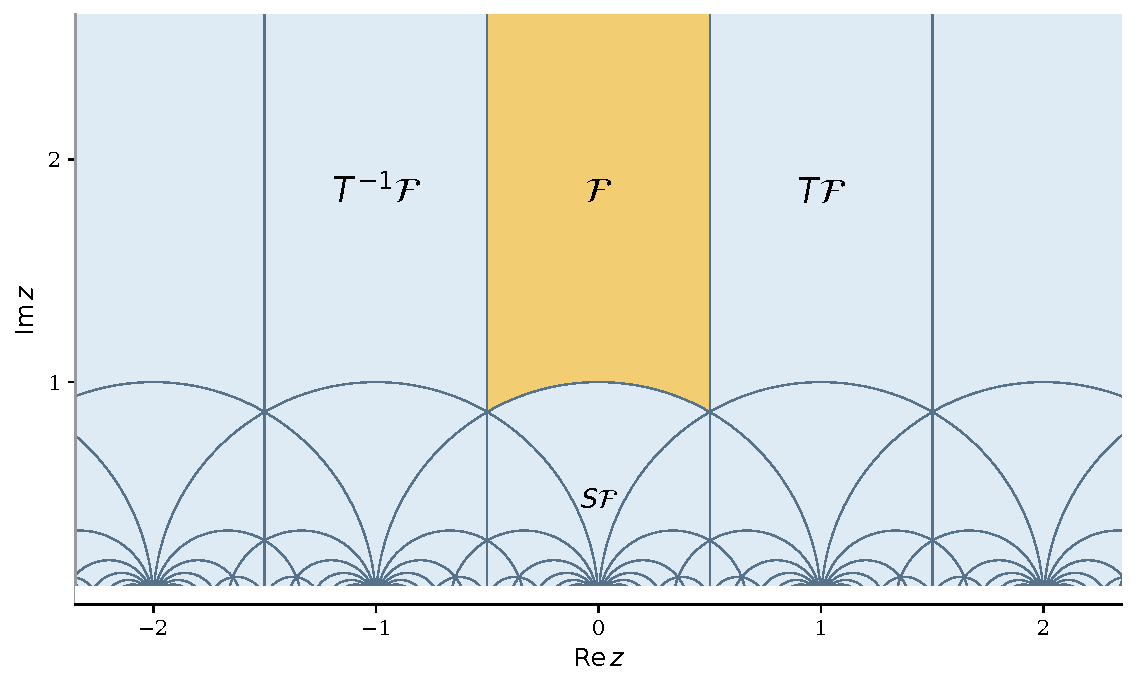
\includegraphics[width=\linewidth]{volumes/Volume01/A/chapters/Chapter01/sections/Section06/figures/modular-tiling.pdf}
\caption{Translates of $\mathcal F$ tile $\mathbb H$. The highlighted domain and its immediate translates $T^{-1}\mathcal F$, $T\mathcal F$, and $S\mathcal F$ are labeled. Every tile is the image under a determinant-one integer matrix; matrices differing by sign give the same tile. Only a finite collection of tiles is drawn, and no completeness at the real boundary is inferred from the drawing.}
\label{modular.tiling-diagram}
\end{figure}

For integration, we can therefore use $\mathcal F$ or its interior with the same result. If an exact representative set for point orbits is wanted, choose
\begin{equation}\label{eq:modular-representative-set}
 \begin{aligned}
 \mathcal F_*={}&\{z\in\mathbb H:-\tfrac12\leq\operatorname{Re}z<\tfrac12,\ |z|>1\}\\
 &{}\cup\{z\in\mathbb H:|z|=1,\ -\tfrac12\leq\operatorname{Re}z\leq0\}.
 \end{aligned}
\end{equation}
The \hyperref[modular.boundary-identifications]{side-pairing proposition} gives exactly one point of each orbit in this set. It does not remove stabilizers at those representatives: stabilizers fix a point rather than produce a different representative of its orbit. We study those stabilizers, the cusp, and the resulting \hyperref[modular.quotient-topology]{quotient topology} in Section 1.7.
